% Practice Test 19 — Alaska Edition
% Questions: 30 (23 MC + 7 SA)
% Generated by scripts/generate_practice_tests.py

\begin{practiceQuestion}{1-3-q01}{mc}
\begin{questionText}
What is the constant of proportionality ($k$) for the table below?

\begin{center}
\begin{tabular}{|c|c|}
\hline $x$ & $y$ \\ \hline $3$ & $12$ \\ $5$ & $20$ \\ $8$ & $32$ \\ \hline
\end{tabular}
\end{center}
\end{questionText}
\choiceA{$3$}
\choiceB{$4$}
\choiceC{$8$}
\choiceD{$12$}
\correctAnswer{B}
\explanation{$k = \frac{y}{x} = \frac{12}{3} = 4$. Check: $\frac{20}{5} = 4$ and $\frac{32}{8} = 4$.}
\end{practiceQuestion}

\begin{practiceQuestion}{1-5-q25}{sa}
\begin{questionText}
A proportional graph shows total cost versus hours of tutoring. The point $(3, 67.50)$ is on the graph. How much does $5$ hours of tutoring cost?
\end{questionText}
\correctAnswer{$\$112.50$}
\explanation{$k = \frac{67.50}{3} = 22.50$ per hour. Cost for $5$ hours: $22.50 \times 5 = \$112.50$.}
\end{practiceQuestion}

\begin{practiceQuestion}{1-6-q16}{mc}
\begin{questionText}
A factory produces $168$ items in $7$ hours. Another factory produces $200$ items in $8$ hours. Which factory is more productive?
\end{questionText}
\choiceA{Factory 1, at $24$ items/hr}
\choiceB{Factory 2, at $25$ items/hr}
\choiceC{They produce the same rate}
\choiceD{Factory 1, at $25$ items/hr}
\correctAnswer{B}
\explanation{Factory 1: $168 \div 7 = 24$ items/hr. Factory 2: $200 \div 8 = 25$ items/hr. Factory 2 is more productive.}
\end{practiceQuestion}

\begin{practiceQuestion}{2-2-q22}{sa}
\begin{questionText}
A school garden has $80$ plants. If $45\%$ are tomato plants, how many tomato plants are there?
\end{questionText}
\correctAnswer{$36$}
\explanation{$\frac{n}{80} = \frac{45}{100}$. Cross-multiply: $100n = 3600$. Divide: $n = 36$ tomato plants.}
\end{practiceQuestion}

\begin{practiceQuestion}{2-5-q01}{mc}
\begin{questionText}
A restaurant bill is $\$40$. You leave a $15\%$ tip. How much is the tip?
\end{questionText}
\choiceA{$\$4.00$}
\choiceB{$\$5.00$}
\choiceC{$\$6.00$}
\choiceD{$\$8.00$}
\correctAnswer{C}
\explanation{$15\% = 0.15$. Tip: $40 \times 0.15 = \$6.00$.}
\end{practiceQuestion}

\begin{practiceQuestion}{3-1-q03}{mc}
\begin{questionText}
Which statement is true?
\end{questionText}
\choiceA{$-5 > -2$}
\choiceB{$-3 > 0$}
\choiceC{$-7 < -4$}
\choiceD{$0 < -1$}
\correctAnswer{C}
\explanation{On a number line, $-7$ is to the left of $-4$, so $-7 < -4$.}
\end{practiceQuestion}

\begin{practiceQuestion}{3-2-q18}{mc}
\begin{questionText}
What value of $n$ makes $(-9) + n = -2$ true?
\end{questionText}
\choiceA{$-11$}
\choiceB{$-7$}
\choiceC{$7$}
\choiceD{$11$}
\correctAnswer{C}
\explanation{$(-9) + n = -2$ means $n = -2 - (-9) = -2 + 9 = 7$.}
\end{practiceQuestion}

\begin{practiceQuestion}{3-3-q21}{sa}
\begin{questionText}
Find the distance between $-11$ and $-3$ on a number line.
\end{questionText}
\correctAnswer{$8$ units}
\explanation{Distance $= |{-11} - (-3)| = |{-11} + 3| = |{-8}| = 8$ units.}
\end{practiceQuestion}

\begin{practiceQuestion}{3-10-q11}{mc}
\begin{questionText}
A pool holds $5{,}400$ gallons. Water drains at $\dfrac{3}{4}$ gallon per minute. How many gallons are left after $2$ hours?
\end{questionText}
\choiceA{$5{,}310$ gallons}
\choiceB{$5{,}310.5$ gallons}
\choiceC{$4{,}500$ gallons}
\choiceD{$5{,}130$ gallons}
\correctAnswer{A}
\explanation{$2$ hours $= 120$ minutes. Drained: $\frac{3}{4} \times 120 = 90$ gallons. Remaining: $5{,}400 - 90 = 5{,}310$.}
\end{practiceQuestion}

\begin{practiceQuestion}{4-1-q02}{mc}
\begin{questionText}
What is the value of $3x - 5$ when $x = 4$?
\end{questionText}
\choiceA{$2$}
\choiceB{$7$}
\choiceC{$17$}
\choiceD{$-2$}
\correctAnswer{B}
\explanation{Substitute: $3(4) - 5 = 12 - 5 = 7$.}
\end{practiceQuestion}

\begin{practiceQuestion}{5-2-q12}{mc}
\begin{questionText}
Solve $\dfrac{w}{5} + 12 = 20$.
\end{questionText}
\choiceA{$w = 40$}
\choiceB{$w = 160$}
\choiceC{$w = 8$}
\choiceD{$w = 1.6$}
\correctAnswer{A}
\explanation{Subtract $12$: $\frac{w}{5} = 8$. Multiply by $5$: $w = 40$. Check: $\frac{40}{5} + 12 = 8 + 12 = 20$ \checkmark.}
\end{practiceQuestion}

\begin{practiceQuestion}{5-3-q21}{sa}
\begin{questionText}
Solve $5(2x - 3) = 35$.
\end{questionText}
\correctAnswer{$x = 5$}
\explanation{Divide by $5$: $2x - 3 = 7$. Add $3$: $2x = 10$. Divide by $2$: $x = 5$. Check: $5(2(5) - 3) = 5(7) = 35$ \checkmark.}
\end{practiceQuestion}

\begin{practiceQuestion}{5-4-q27}{gmc}
\begin{questionText}
Use the fraction bar model to solve: $\dfrac{2}{3}x = 8$. What is $x$?

\begin{center}
\begin{tikzpicture}[scale=0.6]
  % Full bar = x
  \draw[thick,fill=funBlue!15] (0,2) rectangle (12,3);
  \node at (6,2.5) {$x$};
  % 2/3 of bar highlighted
  \draw[thick,fill=funOrange!30] (0,0) rectangle (8,1);
  \node at (4,0.5) {$\frac{2}{3}x = 8$};
  \draw[thick,fill=gray!15] (8,0) rectangle (12,1);
  \node at (10,0.5) {$?$};
  % Dividers
  \draw[dashed] (4,0) -- (4,1);
  \draw[dashed] (4,2) -- (4,3);
  \draw[dashed] (8,0) -- (8,3);
  \node[below] at (2,-0.2) {$\frac{1}{3}$};
  \node[below] at (6,-0.2) {$\frac{1}{3}$};
  \node[below] at (10,-0.2) {$\frac{1}{3}$};
\end{tikzpicture}
\end{center}
\end{questionText}
\choiceA{$x = 12$}
\choiceB{$x = 16$}
\choiceC{$x = 10$}
\choiceD{$x = 5\dfrac{1}{3}$}
\correctAnswer{A}
\explanation{If $\frac{2}{3}x = 8$, then each $\frac{1}{3}$ of $x$ is $4$. So $x = 3 \times 4 = 12$.}
\end{practiceQuestion}

\begin{practiceQuestion}{5-5-q22}{sa}
\begin{questionText}
Solve $8 - 3x \geq 23$.
\end{questionText}
\correctAnswer{$x \leq -5$}
\explanation{Subtract $8$: $-3x \geq 15$. Divide by $-3$ and flip: $x \leq -5$.}
\end{practiceQuestion}

\begin{practiceQuestion}{5-6-q06}{mc}
\begin{questionText}
Solve $-2x \leq 10$ and describe the graph.
\end{questionText}
\choiceA{Closed circle at $-5$, shade left}
\choiceB{Closed circle at $5$, shade left}
\choiceC{Closed circle at $-5$, shade right}
\choiceD{Open circle at $-5$, shade right}
\correctAnswer{C}
\explanation{Divide by $-2$ and flip: $x \geq -5$. Closed circle at $-5$, shade right.}
\end{practiceQuestion}

\begin{practiceQuestion}{6-2-q28}{gmc}
\begin{questionText}
A triangle on Drawing A (scale $1$ cm $= 4$ m) has the dimensions shown below. Drawing B uses scale $1$ cm $= 2$ m. What is the base of the triangle on Drawing B?

\begin{center}
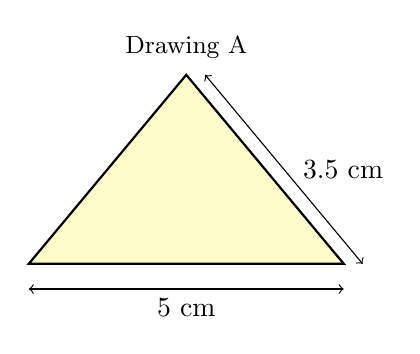
\begin{tikzpicture}[scale=0.8]
  \draw[thick,fill=yellow!20] (0,0) -- (5,0) -- (2.5,3) -- cycle;
  \draw[<->] (0,-0.4) -- (5,-0.4);
  \node[below] at (2.5,-0.4) {$5$ cm};
  \draw[<->] (5.3,0) -- (2.8,3);
  \node[right] at (4.2,1.5) {$3.5$ cm};
  \node[above] at (2.5,3.1) {\small Drawing A};
\end{tikzpicture}
\end{center}
\end{questionText}
\choiceA{$2.5$ cm}
\choiceB{$5$ cm}
\choiceC{$10$ cm}
\choiceD{$20$ cm}
\correctAnswer{C}
\explanation{Scale ratio: $\frac{4}{2} = 2$. New base: $5 \times 2 = 10$ cm.}
\end{practiceQuestion}

\begin{practiceQuestion}{6-3-q14}{mc}
\begin{questionText}
Marcus wants to draw a triangle with angles $60°$, $60°$, and $60°$ and a side of $4$ cm. How many different triangles can he draw?
\end{questionText}
\choiceA{None}
\choiceB{Exactly one}
\choiceC{Exactly three}
\choiceD{Infinitely many}
\correctAnswer{B}
\explanation{AAA with a specified side length fixes the size. A $60°$-$60°$-$60°$ triangle is equilateral, so all sides are $4$ cm. Exactly one triangle.}
\end{practiceQuestion}

\begin{practiceQuestion}{6-4-q13}{mc}
\begin{questionText}
Can a triangle have angles $90°$, $100°$, and $-10°$?
\end{questionText}
\choiceA{Yes, it is a right triangle}
\choiceB{Yes, because the sum is $180°$}
\choiceC{No, because an angle cannot be negative}
\choiceD{No, because the sum is not $180°$}
\correctAnswer{C}
\explanation{Although $90 + 100 + (-10) = 180$, every angle in a triangle must be greater than $0°$. A negative angle is impossible.}
\end{practiceQuestion}

\begin{practiceQuestion}{6-5-q14}{mc}
\begin{questionText}
Which cross-section is NOT possible from slicing a rectangular prism?
\end{questionText}
\choiceA{Rectangle}
\choiceB{Triangle}
\choiceC{Circle}
\choiceD{Pentagon}
\correctAnswer{C}
\explanation{A rectangular prism has flat faces and straight edges. Its cross-sections can be triangles, rectangles, pentagons, or hexagons, but never circles (since it has no curved surfaces).}
\end{practiceQuestion}

\begin{practiceQuestion}{7-3-q09}{mc}
\begin{questionText}
What is the area of a circle with a radius of $10$ cm? Use $\pi \approx 3.14$.
\end{questionText}
\choiceA{$31.4$ cm$^2$}
\choiceB{$62.8$ cm$^2$}
\choiceC{$100$ cm$^2$}
\choiceD{$314$ cm$^2$}
\correctAnswer{D}
\explanation{$A = \pi r^2 = 3.14 \times 100 = 314$ cm$^2$.}
\end{practiceQuestion}

\begin{practiceQuestion}{7-4-q04}{mc}
\begin{questionText}
A shape is made of a square with side $8$ cm and a semicircle with diameter $8$ cm attached to one side. What is the area? Use $\pi \approx 3.14$.
\end{questionText}
\choiceA{$64$ cm$^2$}
\choiceB{$89.12$ cm$^2$}
\choiceC{$114.24$ cm$^2$}
\choiceD{$139.12$ cm$^2$}
\correctAnswer{B}
\explanation{Square: $8^2 = 64$ cm$^2$. Semicircle: $\frac{1}{2} \times \pi r^2 = \frac{1}{2} \times 3.14 \times 16 = 25.12$ cm$^2$. Total: $64 + 25.12 = 89.12$ cm$^2$.}
\end{practiceQuestion}

\begin{practiceQuestion}{7-5-q09}{mc}
\begin{questionText}
A rectangular prism has dimensions $7$ m by $4$ m by $3$ m. What is the area of the largest face?
\end{questionText}
\choiceA{$12$ m$^2$}
\choiceB{$21$ m$^2$}
\choiceC{$28$ m$^2$}
\choiceD{$84$ m$^2$}
\correctAnswer{C}
\explanation{The three pairs of faces have areas $7 \times 4 = 28$, $7 \times 3 = 21$, and $4 \times 3 = 12$ m$^2$. The largest is $28$ m$^2$.}
\end{practiceQuestion}

\begin{practiceQuestion}{7-6-q27}{gmc}
\begin{questionText}
The figure shows unit cubes stacked into an L-shape. Each cube has a side length of $1$ cm. What is the total volume?

\begin{center}
\begin{tikzpicture}[scale=0.45]
  % Bottom row: 5 cubes
  \foreach \x in {0,1,2,3,4} {
    \draw[thick,funBlue,fill=funBlue!10] (\x,0) rectangle (\x+1,1);
  }
  % Second row on left: 3 cubes
  \foreach \x in {0,1,2} {
    \draw[thick,funBlue,fill=funBlue!15] (\x,1) rectangle (\x+1,2);
  }
  % Third row on left: 3 cubes
  \foreach \x in {0,1,2} {
    \draw[thick,funBlue,fill=funBlue!20] (\x,2) rectangle (\x+1,3);
  }
\end{tikzpicture}
\end{center}
\end{questionText}
\choiceA{$8$ cm$^3$}
\choiceB{$11$ cm$^3$}
\choiceC{$15$ cm$^3$}
\choiceD{$33$ cm$^3$}
\correctAnswer{B}
\explanation{Bottom row: $5$ cubes. Second row: $3$ cubes. Third row: $3$ cubes. Total: $5 + 3 + 3 = 11$ cm$^3$.}
\end{practiceQuestion}

\begin{practiceQuestion}{8-1-q22}{sa}
\begin{questionText}
Give one reason why a sample might not perfectly represent a population.
\end{questionText}
\correctAnswer{Random variation (or the sample may be biased)}
\explanation{Even a well-chosen random sample may differ slightly from the population due to chance.}
\end{practiceQuestion}

\begin{practiceQuestion}{8-3-q03}{mc}
\begin{questionText}
When comparing two populations visually, you should look at:
\end{questionText}
\choiceA{Only the center (mean or median)}
\choiceB{Only the spread (range or MAD)}
\choiceC{Both the center and the spread}
\choiceD{Only the largest and smallest values}
\correctAnswer{C}
\explanation{A complete comparison requires looking at both center (where the data clusters) and spread (how spread out it is).}
\end{practiceQuestion}

\begin{practiceQuestion}{8-4-q13}{mc}
\begin{questionText}
Store A daily sales: mean $\$500$, MAD $\$40$. Store B daily sales: mean $\$620$, MAD $\$40$. The difference in means in MADs is:
\end{questionText}
\choiceA{$1.5$ MADs}
\choiceB{$3$ MADs}
\choiceC{$40$ MADs}
\choiceD{$120$ MADs}
\correctAnswer{B}
\explanation{Difference $= \$620 - \$500 = \$120$. In MADs: $\frac{120}{40} = 3$ MADs.}
\end{practiceQuestion}

\begin{practiceQuestion}{8-7-q16}{mc}
\begin{questionText}
A line graph shows a plant's height each week: Week 1: $2$ cm, Week 2: $5$ cm, Week 3: $9$ cm, Week 4: $14$ cm. Between which weeks did the plant grow the most?
\end{questionText}
\choiceA{Week 1 to Week 2}
\choiceB{Week 2 to Week 3}
\choiceC{Week 3 to Week 4}
\choiceD{Growth was the same each week}
\correctAnswer{C}
\explanation{Week 1--2: $3$ cm. Week 2--3: $4$ cm. Week 3--4: $5$ cm. The most growth was Week 3 to 4.}
\end{practiceQuestion}

\begin{practiceQuestion}{9-4-q07}{mc}
\begin{questionText}
A coin is weighted so that heads comes up $60\%$ of the time. What is the probability of tails?
\end{questionText}
\choiceA{$0.60$}
\choiceB{$0.50$}
\choiceC{$0.40$}
\choiceD{$0.30$}
\correctAnswer{C}
\explanation{$P(\text{tails}) = 1 - 0.60 = 0.40$. Since heads and tails have different probabilities, this is a non-uniform model.}
\end{practiceQuestion}

\begin{practiceQuestion}{9-6-q30}{gsa}
\begin{questionText}
Look at the tree diagram for flipping three coins. What is the probability of getting exactly $2$ tails? Write your answer as a fraction in simplest form.

\begin{center}
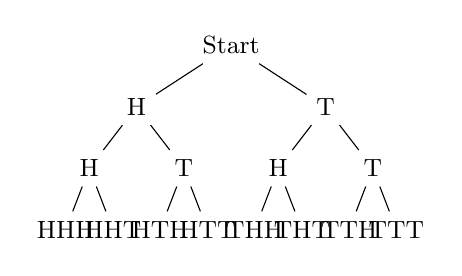
\begin{tikzpicture}[scale=0.6,
  level 1/.style={sibling distance=4cm, level distance=1.3cm},
  level 2/.style={sibling distance=2cm, level distance=1.3cm},
  level 3/.style={sibling distance=1cm, level distance=1.3cm}]
  \node {\small Start}
    child {node {\small H}
      child {node {\small H}
        child {node {\small HHH}}
        child {node {\small HHT}}
      }
      child {node {\small T}
        child {node {\small HTH}}
        child {node {\small HTT}}
      }
    }
    child {node {\small T}
      child {node {\small H}
        child {node {\small THH}}
        child {node {\small THT}}
      }
      child {node {\small T}
        child {node {\small TTH}}
        child {node {\small TTT}}
      }
    };
\end{tikzpicture}
\end{center}
\end{questionText}
\correctAnswer{$\frac{3}{8}$}
\explanation{Outcomes with exactly $2$ tails: HTT, THT, TTH — that is $3$ out of $8$. $P = \frac{3}{8}$.}
\end{practiceQuestion}

\begin{practiceQuestion}{9-7-q17}{mc}
\begin{questionText}
A student wants to simulate the probability that exactly $2$ out of $3$ students pass a test, where each student has a $50\%$ chance. Which model would work?
\end{questionText}
\choiceA{Roll one die: odd = pass, even = fail}
\choiceB{Flip $3$ coins: heads = pass, tails = fail; count exactly $2$ heads}
\choiceC{Draw $3$ marbles from a bag of $2$ red and $1$ blue}
\choiceD{Flip $1$ coin $3$ times and count all tails}
\correctAnswer{B}
\explanation{Each coin flip has a $50\%$ chance of heads (pass). Flipping $3$ coins and counting exactly $2$ heads simulates exactly $2$ passes.}
\end{practiceQuestion}
